
\documentclass{article}
\usepackage{amsmath,amssymb}
\usepackage{graphicx}
\usepackage{array}
\usepackage{wrapfig}
\usepackage{corl_2026} % Use this for the initial submission.
% \usepackage[final]{corl_2026} % Uncomment for the camera-ready ``final'' version.
% \usepackage[preprint]{corl_2026} % Uncomment for pre-prints (e.g., arxiv); This is like ``final'', but will remove the CORL footnote.

\title{S2A2: Audio-Visual Imitation Learning for Manipulation Tasks Using Acoustic Spatial Information}

\author{
  Kaneyoshi Hiratsuka\\
  Kyoto University \\
  Japan\\
  \texttt{hiratsuka.kaneyoshi.i62@kyoto-u.jp} \\
  \And
  Ryosuke Kojima \\
  Kyoto University, RIKEN \\
  Japan \\
  \texttt{email} \\
  \AND
  Benjamin Yen \\
  RIKEN, Institute of Science Tokyo \\
  Japan \\
  \texttt{email} \\
}

\begin{document}
\maketitle
\begin{abstract}

Acoustic information provides rich cues about object location, material properties, and changes caused by contact or motion.
This paper introduces a new set of acoustic-aware manipulation tasks for imitation learning, in which robots must use auditory cues to determine manipulation targets.
These tasks require sound source localization and identification for active exploration in robotic manipulation.
Also, we propose a multimodal imitation learning framework, Spatial-Spectral Audio Action (S2A2), that integrates visual features with acoustic spatial and acoustic signal information for the acoustic-aware manipulation tasks. 
We implemented S2A2 models that integrates policies such as ACT, Diffusion Policy, VQ-BeT, and $\pi_0$, into our framework. Simulation experiments showed that the proposed method is the most effective for tasks requiring both position and timbre.
Furthermore, real-robot experiments confirm the applicability of the proposed tasks and framework to real-world manipulation.

\end{abstract}
\keywords{Multimodal Imitation Learning, Robot Manipulation, Robot Audition, Sound Source Localization}
\section{Introduction}
人間のデモンストレーションから操作方策を獲得する模倣学習は，ロボットが複雑なマニピュレーション技能を獲得するための有力な枠組みとして広く研究されてきた~\citep{pomerleau1988alvinn,argall2009survey,osa2018algorithmic}．
近年では，深層学習の発展により，画像観測やロボット状態から高次元かつ連続的な行動を直接予測する方策学習が可能となり，物体操作，接触を伴う作業，双腕操作など，多様なロボットマニピュレーションへ応用されている~\citep{vla_survey2025}．

しかし，既存の模倣学習タスクの多くは，タスクの操作対象が視覚的に観測可能であり，目的も視覚的な対応付けができることを暗黙に仮定している．
この仮定は，照明変動，オクルージョン，外観が同一または類似した複数物体が存在する状況，あるいは物体の内部状態や発生イベントが画像上に現れない状況では破綻し得る~\citep{playitbyear}．
このような部分観測性を緩和するため，視覚に加えて触覚や音響などのモダリティを統合する研究が進められている~\citep{seehearfeel,vtt2022,sts_il2024,vitamin2024,tacthru2025,neuralfeels2024}．

本研究では，その中でも，物体の外観には現れない多様な情報が含まれるacoustic informationに着目する．
接触音や衝突音は物体の材質や接触状態を反映し~\citep{seehearfeel,thatsoundsright,hearingtouch2024,maniwav,multigen2025}，注ぐ，振る，流れるといった相互作用に伴う音は，粒状物質の量や流量~\citep{clarke2018learning,wilson2019pouring}，液体の高さ~\citep{liang2020audiopouring,du2021robotpouring}などを推定する手がかりとなる．
さらに，ロボットは物体を振る，叩く，擦るといった能動的探索行動を通じて，視覚だけでは得られない音響的手がかりを自ら引き出すこともできる~\citep{eppe2018interactive,caver2025,mosaic2024}．
重要なのは，acoustic informationが「何が起きているか」というsignal informationだけでなく，「どこで起きているか」というspatial informationも同時に持ち得る点である．

この性質は，従来の視覚中心のマニピュレーションとは異なる新しいタスク設定を生み出す．
例えば，外観が同一の複数物体の中から音を発している物体を選ぶ，音色に基づいて物体状態や搬送先を決定する，あるいはロボット自身が物体を振ることで音響手がかりを取得し次の行動を決める場合，方策は視覚的な物体配置だけでなく，acoustic spatial informationとacoustic signal informationを統合して行動を生成する必要がある．
本研究では，このように，空間的に分布した音環境が操作対象の選択，ゴールの決定，または能動的探索に直接関与するタスク群を，acoustic-aware manipulation tasksとして導入する．

既存の音響を用いたロボットマニピュレーション研究は，主に接触マイクや単一マイクから得られるspectrogramを用いて，音色，接触イベント，物体状態を識別することに焦点を当ててきた~\citep{playitbyear,seehearfeel,maniwav,hearingtouch2024,audiovla}．
一方，マイクロフォンアレイを用いた音源定位・追跡・分離技術を中心としたロボット聴覚の分野では，ロボットにおける対話，ナビゲーション，音源追跡を対象としている一方，マニピュレーション方策への統合は限定的である~\citep{nakadai2020robotaudition,robotaudition_review2025}．

その為，本研究では，acoustic spatial informationを表すacoustic spatial mapと，acoustic signal informationを表すspectrogramを視覚情報と統合するSpatial-Spectral Audio Action (S2A2) frameworkを提案する．
本提案手法では，具体的に，定位情報としてMUSIC法~\citep{schmidt1986music,doa_survey2025}に基づいて音源位置の尤度に対応したacoustic spatial mapとその位置のacoustic signal informationを強調するSpotforming~\citep{spotforming_nmf}により抽出したspectrogramと組み合わせることで，音が「どこで」「どのように」発生しているかを方策が利用できることが期待できる．

本実験では，上述の，acoustic-aware manipulation tasksに対し，
S2A2 frameworkを用いた手法を適用し，マニピュレータロボットと複数マイクロフォンアレイのシミュレーション・及び実機を用いて評価を行い，音響の空間的な表現が現実のマニピュレーションにおいて有効に機能することを検証する．

本研究の貢献は次の三点である．

\begin{itemize}
	\item 空間的に分布した音環境が操作対象の選択，ゴールの決定，能動的探索に関与するacoustic-aware manipulation tasksを新たに導入する．
	\item acoustic spatial informationとacoustic signal informationを視覚情報と統合するマルチモーダル模倣学習フレームワークS2A2を提案する．
	\item acoustic-aware manipulation tasksを通じて，acoustic informationが方策学習に与える寄与を系統的に評価し，シミュレーションおよび実機環境の双方でS2A2 frameworkを評価する．
\end{itemize}

	\begin{figure}[t]
		\centering
		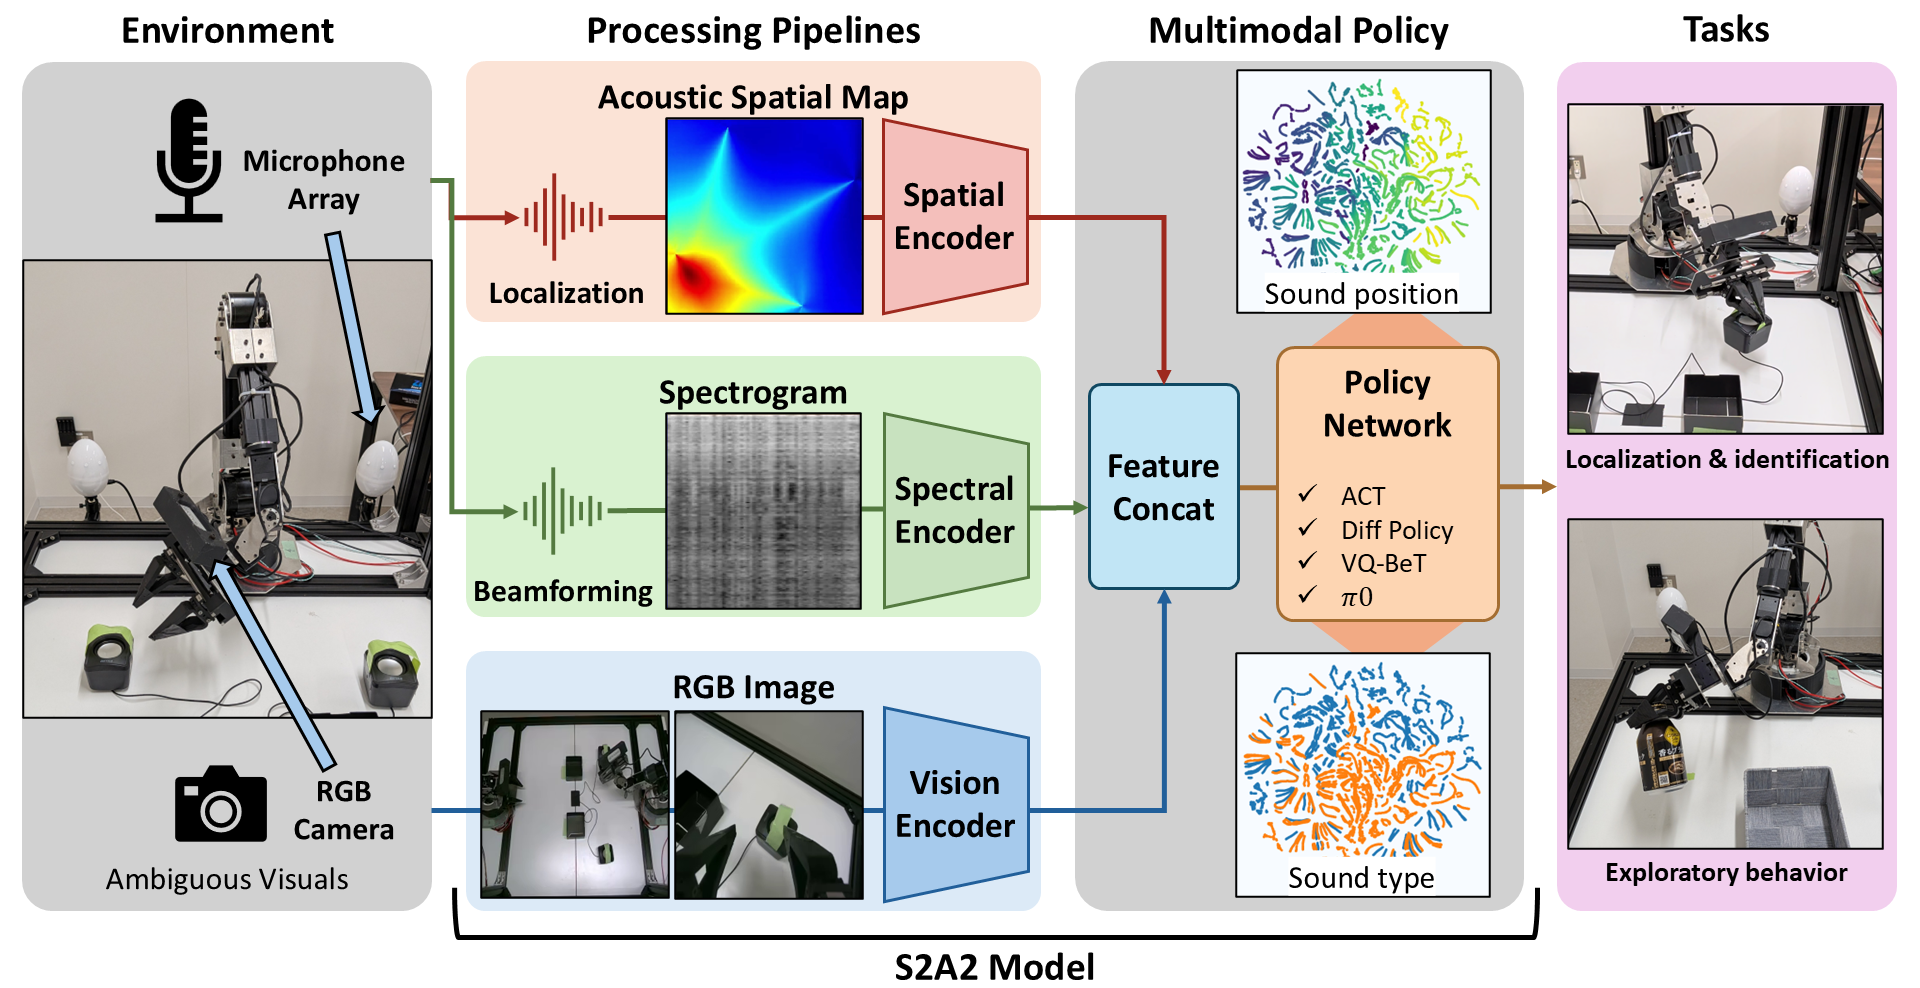
\includegraphics[keepaspectratio, width=14cm]{fig/fig1.png}
		\caption{The Overview of S2A2 framework.
		RGBカメラから得られる画像はVision Encoderによって特徴量を抽出される．同様に，複数のマイクロフォンアレイから得られる多チャンネルacoustic informationからは，acoustic spatial mapとspectrogramを生成し，それぞれ専用エンコーダで特徴量化する．これらの画像，acoustic featuresを統合し，ACT，Diffusion Policy，VQ-BeT，$\pi_0$の4種の模倣学習Policyへ入力することで，音の識別であったり音の探索といった行動生成を可能にする．}
		\label{fig:fig1}
	\end{figure}
\section{Related Work}
	本研究は，模倣学習，manipulation with acoustic modality，robot audition with microphone array processingの3領域にまたがるため，
	本節では，これらの各領域における関連研究について述べる．

\subsection{Imitation Learning and Multimodal Manipulation}
近年の深層模倣学習では，高次元観測から連続的な行動系列を生成するため，方策表現の高度化が進んでいる~\citep{rmp_survey2025}．
ACT~\citep{act}はTransformer~\citep{vaswani2017attention}と条件付きVAEにより行動系列をチャンクとして予測し，Diffusion Policy~\citep{diffusionpolicy}は拡散モデル~\citep{ho2020ddpm}を用いてマルチモーダルな行動分布をdenoising過程として表現する．
VQ-BeT~\citep{vqbet}は連続行動を離散コードへ量子化し，Decoder-only Transformerで自己回帰的に予測することで長期的な行動構造を扱う．
また，$\pi_0$~\citep{pi0}はPaliGemma~\citep{beyer2024paligemma}を基盤とし，flow matching~\citep{lipman2023flow}により行動系列を生成する．
これらは，行動の時間構造や分布のマルチモダリティを扱う代表的な方策学習手法である．

一方，入力モダリティの観点では，多くの手法は視覚を主入力としており，RT-2~\citep{brohan2023rt2}やOpenVLA~\citep{kim2024openvla}などのVision-Language-Actionモデルも，視覚と言語によるタスク指定を行動生成へ接続することで汎用的な操作方策を目指している~\citep{vla_survey2025}．
しかし，操作に必要な情報が外観に現れない場合や，外観上区別できない物体を扱う場合には，視覚・言語のみでは物理的な曖昧性を十分に解消できない．

この制約を補うため，視覚以外のセンサモダリティを模倣学習へ統合する研究も進んでいる．
特に触覚は，接触後の力学的状態や局所的な物体情報を捉える上で有効であり，視触覚を統合したpolicyは，密なパッキング~\citep{seehearfeel}，接触に富む操作~\citep{vtt2022,sts_il2024,vitamin2024,tacthru2025}，掌上操作~\citep{neuralfeels2024}などで視覚のみのpolicyを上回ることが報告されている．
触覚や言語と本研究で扱う音響表現は競合するものではなく，将来的にはこれらと組み合わせることで，より多様なマルチモーダル操作へ拡張できる可能性がある．

\subsection{Manipulation with Acoustic Modality}
音響モダリティは，材料識別~\citep{eppe2018interactive,jin2019openenv}，粒状物質の流量や量の推定~\citep{clarke2018learning,wilson2019pouring}，液体の高さ推定~\citep{liang2020audiopouring,du2021robotpouring}など，多くの認識タスクで利用されてきた．
ロボット操作への応用としては，接触音を用いた方策学習~\citep{seehearfeel,maniwav}や動作生成~\citep{thatsoundsright}が提案されており，さらに大規模音響データセットによる事前学習~\citep{hearingtouch2024}やVLAとの統合~\citep{audiovla}も研究されている．

接触音に限らずacoustic informationに着目した研究として，The Sound of Simulation~\citep{multigen2025}は生成モデルによる音響データ拡張を用いたsim-to-real方策学習を扱い，CAVER~\citep{caver2025}とMOSAIC~\citep{mosaic2024}は能動的探索とacoustic informationの統合を扱う．
また，Play it by Ear~\citep{playitbyear}は遮蔽下の操作において視覚と音を併用している．
一方で，既存研究の多くはグリッパ近傍や接触マイクから得られる単一チャンネル音を利用しており，マイクロフォンアレイにより音環境を空間的に捉えるモダリティの活用は限定的である．


\subsection{Robot Audition and Microphone array Processing}
ロボット聴覚の分野では，ロボットが活動する環境ノイズ下においてマイクロフォンアレイを用いて音源定位・追跡・分離を実現する研究がされてきた~\citep{nakadai2020robotaudition,robotaudition_review2025}．
それに関連して，複数のマイクロフォンアレイを用いる研究も多くされており，非同期なマイクロフォンアレイを使用してのキャリブレーション~\citep{wang2024slamcalib}，仮想空間での音響シーンの再現\cite{gabriel20192d}，音源の追跡\citep{yamada2020sound}などが行われている．
特に，複数アレイとNMFを組み合わせたSpotforming~\citep{spotforming_nmf}は，対象領域に対応する音源を強調し，周囲雑音や同方向雑音を抑制する枠組みを提供する．
本研究は，これらのロボット聴覚技術をマニピュレーション模倣学習の文脈に接続した最初の研究であるとも位置付けることができる．

\section{Spatial-Spectral Audio Action (S2A2) framework}
\label{sec:s2a2_framework}

	Fig.~\ref{fig:fig1}に示すように，S2A2 frameworkは，環境設定，S2A2 model，およびacoustic-aware manipulation tasksから構成される．
	S2A2 modelは，観測からモダリティ別に特徴量を抽出するprocessing pipelinesと，それらを統合して次の行動を出力する multimodal policy から構成される．
	
	% 本章の構成は以下の通りである．
	% まず，Section~\ref{sec:problem}でS2A2 frameworkの問題設定および模倣学習としての定式化を行う．
	% 次に，Section~\ref{sec:tasks}で本研究が対象とする具体的なタスクについて述べる．
	% Section~\ref{sec:pipelines}では，S2A2 modelを構成する3つの processing pipelinesにおける前処理アルゴリズムとエンコーダの構造を説明する．
	% 最後に，Section~\ref{sec:policy}でmultimodal policyによる特徴量の統合と次の行動の決定について述べる．

\subsection{Problem Formulation}
\label{sec:problem}
S2A2 frameworkは，視覚のみでは操作対象や搬送先を一意に決定できないacoustic-aware manipulation tasksを対象とし，視覚情報に加えてacoustic spatial informationおよびacoustic signal informationを利用して行動を決定する．

本研究では，この問題を視覚・聴覚観測に条件づけられた模倣学習問題として定式化する．各時刻の観測$o_t$は，RGB画像$\mathbf{I}_t$，多チャンネルacoustic information $A_t$，proprioception $s_t$から構成され，$A_t$からacoustic spatial map $S_t$とspectrogram $G_t$を得る．
S2A2 modelは，これらの観測に基づき，$H$ステップ先までの行動列$a_{t+H-1}$を予測するpolicy $\pi_\theta$を学習する．学習では，エキスパート軌道から得られたデータセット$\mathcal{D}$に対して，予測行動とエキスパート行動のずれを表す模倣学習損失$\mathbb{E}_{(o_t,a_{t:t+H-1})\sim\mathcal{D}}
	\left[\mathcal{L}_{\mathrm{BC}}\left(\pi_\theta(o_t),a_{t:t+H-1}\right)\right]$を最小化する．
具体的な損失関数は policy network 手法に依存し，その詳細はSection~\ref{sec:policy}およびAppendix~\ref{sec:appendix_architecture}で述べる．


	% S2A2 frameworkは，視覚のみでは正しい操作対象や搬送先を一意に決定できない環境におけるマニピュレーションタスクであるacoustic-aware manipulation tasksを対象とする(詳細はSection~\ref{sec:tasks}で述べる)．
	% このような環境では，ロボットは物体の見た目だけでなく，acoustic spatial informationやacoustic signal informationを利用して行動を決定する必要がある．

	% S2A2 frameworkでは，この問題を視覚と聴覚の観測に条件づけられた模倣学習問題として定式化する．
	% 各時刻$t$における観測$o_t=(\mathbf{I}_t,A_t,s_t)$は，RGB画像 $\mathbf{I}_t$，多チャンネルacoustic information$A_t$，および関節角度やエンドエフェクタの姿勢などのロボット自体の状態を指す proprioception ベクトル$s_t$から構成される．
	% また，多チャンネルacoustic information$A_t$を処理する事で得られる，中間的なacoustic informationとして，音源の空間的位置を表すacoustic spatial map $S_t$（Section~\ref{sec:doa}で詳細を説明），対象の音源のspectrogram $G_t$ (Section~\ref{sec:spec}で詳細を説明)を導入する．

	% S2A2 modelは，これらの観測から$H$ステップ先までの将来の行動列$a_{t:t+H-1}$を予測する policy $\pi_\theta$のパラメータ$\theta$を学習する．
	% データセットをエキスパートによる観測・行動軌道 $\mathcal{D}=\{(o_t,a_{t:t+H-1})\}_t$ とすると，学習の目的は次の模倣学習損失を最小化することである．

	% \begin{equation}
	% \min_{\theta}\ \mathbb{E}_{(o_t,a_{t:t+H-1})\sim\mathcal{D}}
	% \left[\mathcal{L}_{\mathrm{BC}}\left(\pi_\theta(o_t),a_{t:t+H-1}\right)\right],
	% \end{equation}

	% ここで $\mathbb{E}_{(o_t,a_{t:t+H-1})\sim\mathcal{D}}[\cdot]$ はデータセット $\mathcal{D}$ からサンプルした観測・行動ペアに関する期待値，$\pi_\theta(o_t)$ はpolicyが観測 $o_t$ から予測する行動，$\mathcal{L}_{\mathrm{BC}}$ はエキスパート行動とのずれを測る模倣学習損失である．
	% 具体的な損失関数は policy network 手法に依存し，その詳細はSection~\ref{sec:policy}およびAppendix~\ref{sec:appendix_architecture}で述べる．

\subsection{Acoustic-Aware Manipulation Tasks}
\label{sec:tasks}
本研究では，acoustic informationが操作判断に果たす役割を評価するため，acoustic-aware manipulation tasksと名付けた4種類のマニピュレーションタスクを用いる．
各タスクの概要をTable~\ref{tab:tasks}に示す．
いずれのタスクにおいても，環境中には操作対象となる物体と搬送先となる箱が配置され，マニピュレータは適切な物体を把持し，指定された箱へ投入することが求められる．
また，物体の初期位置はランダムに設定される一方で，箱の初期位置は固定される．

\textbf{Localization task}では，
視覚的に区別できない2つの物体を用い，2つの物体のうち一方のみが常時音を発し，マニピュレータは音を発している物体を把持して箱に入れる．
発せられる音は，全エピソードを通じて単一の音を使用するため，把持対象の選択に必要となる情報は音源の空間的位置である．

\textbf{Identification task}では，1つの物体と2つの箱を用いる．
物体は常時2種類の音のいずれかを発し，マニピュレータはその音に対応する箱へ物体を搬送する．
この時，各音に対応する箱の位置は全エピソードを通して共通である．
音を発する物体は1つであるため，視覚情報により把持対象は一意に定まり，acoustic spatial informationは不要である．
一方で，適切な搬送先を選択するためには音の識別が必要となる．

\textbf{Localization \& identification task}(L\&I Task)では，視覚的に区別できない2つの物体と2つの箱を用いる．
2つの物体のうち一方のみが常時音を発し，その音は2種類の音のいずれかである．
マニピュレータは，acoustic spatial informationに基づいて把持対象を特定し，さらに音に基づいて対応する箱へ搬送する．
この時，各音に対応する箱の位置は全エピソードを通して共通である．
このように，本タスクでは対象物体の選択に音源定位が，搬送先の選択に音の識別がそれぞれ必要となる．

\textbf{Exploratory task}では，視覚的に区別できない2つの物体と1つの箱を用いる．
いずれの物体も静止時には音を発さず，一方の物体のみを動かした時に音を発する．
マニピュレータは，2つの物体を順に把持して振ることで音の有無を確認し，音を発した物体を箱に入れる必要がある．


\begin{wraptable}{r}{0.48\textwidth}
  \centering
  \setlength{\tabcolsep}{3pt}
  \caption{
	%Acoustic-Aware Manipulation Task の各タスクが要求する音響的能力．
	Acoustic capabilities relevant to each task in the acoustic-aware manipulation task.
	}
  \label{tab:tasks}
  \begin{tabular}{p{0.15\textwidth} p{0.09\textwidth}
    >{\centering\arraybackslash}p{0.09\textwidth}
    >{\centering\arraybackslash}p{0.09\textwidth}}
    \hline
    Task & Space & Signal & Explore \\
    \hline
    Localization & $\checkmark$ & -- & -- \\
    Identification & -- & $\checkmark$ & -- \\
    L\&I & $\checkmark$ & $\checkmark$ & -- \\
    Exploratory & $\checkmark$ & $\checkmark$ & $\checkmark$ \\
    \hline
  \end{tabular}
\end{wraptable}



	% \begin{table*}[t]
	% 	\centering
	% 	\scriptsize
	% 	\setlength{\tabcolsep}{3pt}
	% 	\caption{acoustic-aware manipulation tasksの各タスクが要求する音響的能力．}
	% 	\label{tab:tasks}
	% 	\begin{tabular}{p{0.2\textwidth} p{0.3\textwidth} >{\centering\arraybackslash}p{0.15\textwidth} >{\centering\arraybackslash}p{0.2\textwidth}}
	% 		\hline
	% 		Task & Object selection & Goal selection & Requires active interaction \\
	% 		\hline
	% 		Localization task & sound location & not required (single) & no\\
	% 		Identification task & not required (single) & sound timbre & no\\
	% 		L\&I task & sound location & sound timbre & no\\
	% 		Exploratory task & sound presence (after shaking) & not required (single) & yes\\
	% 		\hline
	% 	\end{tabular}
	% \end{table*}

\subsection{Processing Pipeline}
\label{sec:pipelines}

S2A2 modelは，acoustic spatial information，acoustic signal information，視覚情報を処理する3つのpipelineを持つ．
各pipelineは入力モダリティに応じた前処理とエンコーダから構成される．
本節では，既存研究におけるpolicyのvision encoderを直接用いるRGB image pipelineを除き，acoustic spatial map pipelineとspectrogram pipelineについて述べる．

\subsubsection{Acoustic Spatial Map Pipeline}
\label{sec:doa}
	本研究ではFig.~\ref{fig:fig2}に示すように，全マイクロフォンアレイを作業空間と同一平面上に配置する．
	acoustic spatial map pipelineでは，マイクロフォンアレイで収録した多チャンネルacoustic informationから音源方向の尤度を推定し，それを作業空間に対応する二次元マップへ投影する．
	具体的には各マイクロフォンアレイの多チャンネル信号に対し，multiple signal classification (MUSIC) 法~\citep{schmidt1986music}を適用する．
	入力音声信号はサンプリング周波数16kHzで取得し，FFT長512，50\%オーバーラップの短時間フーリエ変換 (STFT) で周波数領域へ変換する．
	
	%各アレイのマイクロフォン数 $M$ 
	方向ごとの空間スペクトルを対数化および正規化した値をdirection of arrival (DOA) スコアとし，これをアレイ中心からの距離に応じた減衰項を導入したうえで，作業空間のマイクロフォンアレイが存在する平面に対応した $224\times224$ の二次元平面へ投影し，アレイの数を$N$としてのacoustic spatial map $S\in\mathbb{R}^{224\times224\times N}$を計算する．処理の詳細については Appendix~\ref{sec:app_doa}．
	このacoustic spatial map $S$ を，spatial encoder に入力し，policy networkが利用できる特徴量に変換する．
	spatial encoder のアーキテクチャは入力チャンネル数を $N$ に拡張したResNet-18を使用し，scratchから学習し，出力としてfeature mapを得る．
	

\subsubsection{Spectrogram Pipeline}
\label{sec:spec}
	spectrogram pipelineでは，対象音源のacoustic signal informationを抽出するためのpipelineである．
	まずacoustic spatial map $S$より，音源の存在尤度を計算し，それに対しピーク抽出を行い音源候補として選択する．
	ここでは，同時に存在する音源の数が1つであるため，最も高いピークを音源候補とした．
	音源候補に対し，Spotforming~\citep{spotforming_nmf}法を利用して音源分離を行い，spectrogramを生成する．処理の詳細については Appendix~\ref{sec:app_doa}．
	このspectrogram を，spectral encoder に入力し，policy network が利用できる特徴量に変換する．
	spectral encoderには，入力チャンネル数を1に変更したResNet-18をscratchから学習する．


\subsection{Multimodal Policy}
\label{sec:policy}
	multimodal policyは，processing pipelinesから抽出された各モダリティの特徴量とproprioceptionを統合し，ロボットの行動を生成するモジュールである．

	本研究では，行動生成を行うpolicy networkとしてACT~\citep{act}，Diffusion Policy~\citep{diffusionpolicy}，VQ-BeT~\citep{vqbet}，および$\pi_0$~\citep{pi0}の4種類を採用した．
	主要な設計方針として，これらの既存policy networkを最小限の変更で，音響表現を各policyが扱えるトークンまたは条件ベクトルへ変換し，RGB画像やproprioceptionとシームレスに統合できるように拡張を施している．

	Section~\ref{sec:pipelines}で述べたように，各pipelineは共通してfeature mapを出力する．
	一方で，得られたfeature mapをpolicy networkへ入力する形式は，各policyの構造に応じて異なるが，各policy networkの詳細はAppendix~\ref{sec:appendix_architecture}に記載した．

\section{Experiments}
\label{sec:result}
	%本章では，まず~\ref{sec:sim_setup}節でシミュレーション環境と評価手順を述べ，~\ref{sec:sim_results}節で定量・定性的な実験結果を報告し，~\ref{sec:real}節で実機実験による検証を行う．


\subsection{シミュレーション実験結果}
\label{sec:sim_results}
    
	ここでは，まず，S2A2フレームワーク内の processing pipelinesと
	~\ref{sec:tasks}節で定義した acoustic-aware manipulation tasksの関係を調べるためのシミュレーション実験を行う．
	本実験ではprocessing pipelineの組合せを変化させて以下の4条件を比較する．
	  (\textbf{Baseline}) RGB image pipelineのみを使用し，acoustic informationを一切利用しない条件．
	(\textbf{S2A2}) 3つのprocessing pipelinesをすべて用いる提案手法の標準条件．
	(\textbf{w/o Spec.}): S2A2 modelからspectrogram pipelineを除き，RGB image pipelineの視覚情報と，acoustic spatial mapによるacoustic spatial informationを利用する条件．
	(\textbf{w/o Spat.}): S2A2 modelからacoustic spatial map pipelineを除き，RGB image pipelineの視覚情報と，spectrogramによるacoustic signal informationを利用する条件．
	ただし，いずれの条件でもmultimodal policyの構造は共通であり，各pipelineの出力する特徴量を結合してpolicy networkに入力する点は変わらない．
	Fig.~\ref{fig:fig2}に示すように，物理シミュレータGenesis~\citep{Genesis}と音響シミュレータPyroomacoustics~\citep{pyroomacoustics}を統合したシミュレーション環境を構築する（詳細はAppendix~\ref{sec:app_simu}）．
	その他の最適化設定とモデル内部パラメータはAppendix~\ref{sec:appendixA}にまとめる．各タスクは3つの異なる乱数シードで学習し，評価指標は100回の試行において700ステップに相当する約23秒以内に，正しい物体を把持し，正しい箱に投入した割合とした．

	\begin{figure}[t]
		\centering
		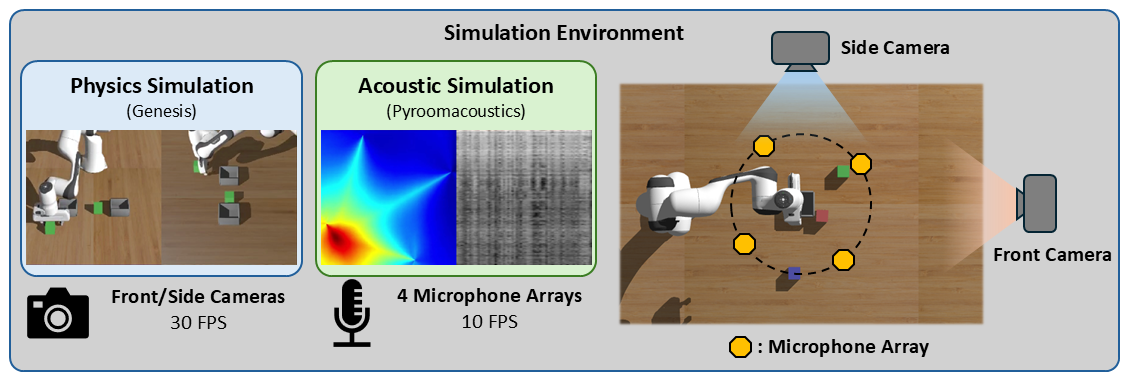
\includegraphics[keepaspectratio, width=14cm]{fig/fig2.png}
		\caption{Simulation settings: 物理シミュレータGenesisと音響シミュレータPyroomacousticsを統合したシミュレーション環境構成．カメラから取得されるRGB画像は30FPSで，microphone arrayから取得されるacoustic informationは10FPSで更新される．Franka Emika Pandaの500mm正面を作業空間の中心とし，その中心から半径300mmの円周上に4つのマイクロフォンアレイを等間隔に配置した．side cameraとfront cameraの2台のカメラは作業空間の中心を映すように設置した．}
		\label{fig:fig2}
	\end{figure}


\begin{figure}[t]
		\centering
		\includegraphics[keepaspectratio, width=14cm]{fig/fig3_new.png}
		\caption{学習ステップ数に対するタスク成功率の変化．4タスクにおけるS2A2 modelの4 policy（ACT，Diffusion Policy，VQ-BeT，$\pi_0$）における学習推移を示す．localization taskおよびidentification taskは10,000 Step毎に最大100,000 Stepまで，L\&I taskおよびexploratory taskは20,000 Step毎に最大200,000 Stepまで評価した．}
		\label{fig:fig3}
\end{figure}



	\begin{table*}[t]
		\centering
		\scriptsize
		\setlength{\tabcolsep}{4pt}
		\caption{
			% 全タスクにおけるタスク成功率（\%）の比較（Mean $\pm$ STD）．各policy内で最良の値を太字で示す．
			Comparison of task success rates (\%) across all tasks (Mean $\pm$ STD). The best value within each policy is shown in bold.
			}
		\label{tab:results}
		\begin{tabular}{llcccc}
			\hline
			Model & Policy & localization task & identification task & L\&I Task & exploratory task \\
			\hline
			Baseline & ACT & 20.3 $\pm$ 7.2 & 39.3 $\pm$ 4.0 & 11.0 $\pm$ 3.5 & 35.0 $\pm$ 5.3 \\
			 & Diffusion Policy & 13.3 $\pm$ 1.2 & 41.3 $\pm$ 2.5 & 9.3 $\pm$ 6.1 & 26.3 $\pm$ 0.6 \\
			 & VQ-BeT & 12.7 $\pm$ 6.8 & 24.0 $\pm$ 6.9 & 7.7 $\pm$ 1.2 & 17.3 $\pm$ 5.8 \\
			 & $\pi_0$ & 18.3 $\pm$ 2.3 & 32.3 $\pm$ 2.1 & 7.0 $\pm$ 4.0 & 9.0 $\pm$ 1.0 \\
			\hline
			S2A2 & ACT & 73.0 $\pm$ 5.6 & \textbf{76.7 $\pm$ 1.2} & \textbf{78.7 $\pm$ 2.1} & \textbf{77.3 $\pm$ 5.7} \\
			 & Diffusion Policy & 68.0 $\pm$ 3.6 & 67.7 $\pm$ 7.2 & \textbf{89.7 $\pm$ 2.1} & \textbf{44.0 $\pm$ 3.6} \\
			 & VQ-BeT & 40.3 $\pm$ 4.5 & 32.3 $\pm$ 10.0 & \textbf{55.3 $\pm$ 11.7} & \textbf{32.7 $\pm$ 12.7} \\
			 & $\pi_0$ & \textbf{32.0 $\pm$ 9.9} & 73.3 $\pm$ 8.4 & \textbf{45.7 $\pm$ 8.1} & 18.7 $\pm$ 4.2 \\
			\hline
			w/o Spec. & ACT & \textbf{74.7 $\pm$ 4.7} & 44.3 $\pm$ 2.3 & 45.0 $\pm$ 3.6 & 75.3 $\pm$ 5.0 \\
			 & Diffusion Policy & \textbf{68.3 $\pm$ 13.7} & 32.7 $\pm$ 3.1 & 46.0 $\pm$ 5.3 & 37.3 $\pm$ 8.1 \\
			 & VQ-BeT & \textbf{44.7 $\pm$ 5.5} & 32.7 $\pm$ 3.1 & 32.3 $\pm$ 7.5 & 20.0 $\pm$ 20.0 \\
			 & $\pi_0$ & 17.3 $\pm$ 5.0 & 40.0 $\pm$ 11.4 & 14.3 $\pm$ 2.9 & \textbf{26.7 $\pm$ 3.2} \\
			\hline
			w/o Spat. & ACT & 15.3 $\pm$ 4.0 & 74.3 $\pm$ 7.0 & 25.7 $\pm$ 3.1 & 72.3 $\pm$ 8.4 \\
			 & Diffusion Policy & 15.3 $\pm$ 1.2 & \textbf{80.3 $\pm$ 3.8} & 8.7 $\pm$ 3.8 & 6.3 $\pm$ 2.3 \\
			 & VQ-BeT & 12.3 $\pm$ 3.8 & \textbf{49.3 $\pm$ 9.8} & 19.0 $\pm$ 1.0 & 25.0 $\pm$ 3.6 \\
			 & $\pi_0$ & 14.7 $\pm$ 5.7 & \textbf{78.7 $\pm$ 6.0} & 19.7 $\pm$ 3.8 & 9.3 $\pm$ 10.4 \\
			\hline
		\end{tabular}
	\end{table*}

\subsubsection{タスク成功率の比較}
	Table~\ref{tab:results}は4タスクにわたる成功率を示しており，学習ステップ数に対する成功率の推移をFig.~\ref{fig:fig3}に示す．
	この結果より，全タスクを通じて，タスクが要求する条件と関連するモデルで最良の成功率が得られる傾向が一貫して観察された．
	acoustic spatial informationのみを要するlocalization taskや，acoustic signal informationのみを要するidentification taskでは，それぞれ対応する条件のみのモデル(w/o Spec. and w/o Spat.)がS2A2 modelに並ぶ性能を示す一方，両者を要するL\&I taskでは，両Pipelineを備えるS2A2 model が単独で比較的高いタスク成功率を達成した．
	
	全タスクを通じて，要求される音響情報に対応したモデルが高い成功率を示し，特に空間情報と信号情報の両方を要するL\&I taskではS2A2 modelが有効であった．一方で，タスクに不要なprocessing pipelineを追加すると性能が低下する場合があり，限られたデータ下では冗長な音響入力がpolicy学習を阻害する可能性が示唆された．acoustic informationによる改善幅はpolicyに依存し，ACTとDiffusion Policyでは顕著な改善が見られた一方，VQ-BeTでは改善幅が小さく，$\pi_0$ではタスクによって性能差が大きかった．（Appendix~\ref{sec:results}）

\subsubsection{潜在特徴量の可視化}
\label{sec:visualization}
	Fig.~\ref{fig:fig4}に示すACTやDiffusion Policyの中間層の潜在特徴量をt-SNE~\citep{vandermaaten2008tsne}により2次元へ射影し可視化した結果を示し，タスク成功率との関係を述べる．
	可視化方法および全policyの可視化結果はAppendix~\ref{sec:appendixB}にまとめる．

	\begin{figure}[t]
		\centering
		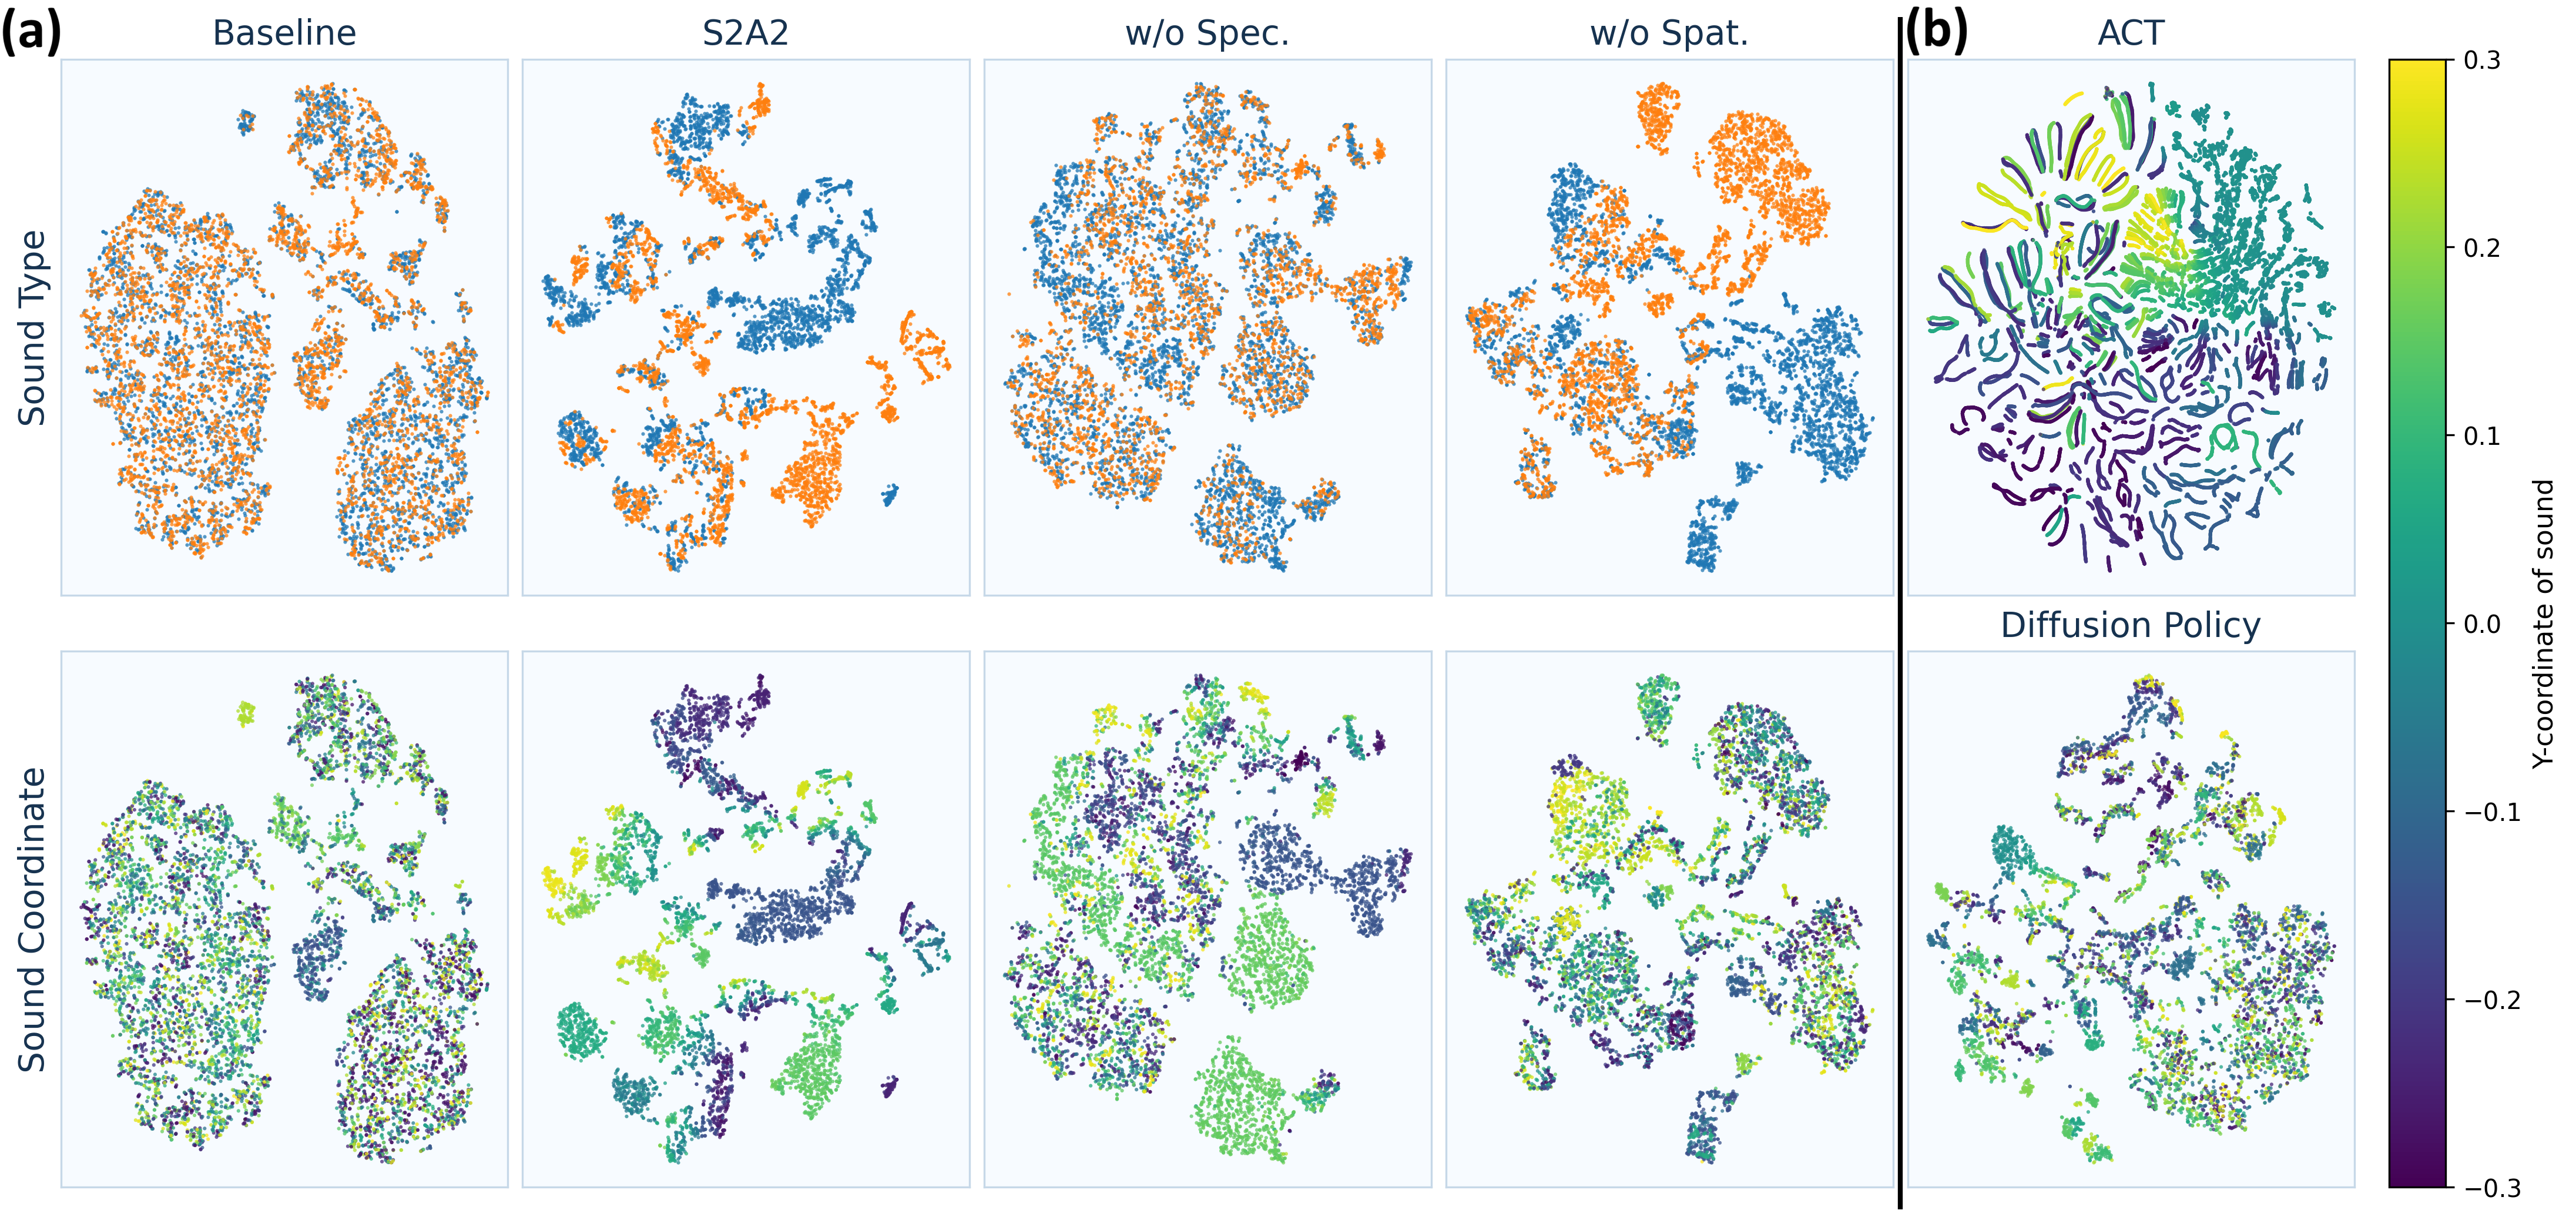
\includegraphics[keepaspectratio, width=14cm]{fig/fig4.png}
		\caption{潜在空間の可視化．(a) Diffusion PolicyのL\&I taskにおける，baseline，S2A2, w/o Spec.，w/o Spat.の比較．t-SNEで分離した潜在特徴量に対して，上段は物体が鳴らしていた音の種類で色分けした図であり，下段は音を鳴らしていた物体のY座標をカラーマップで表現した図．上段の図において，音Aはオレンジ，音Bは青色の点で表現した．(b) exploratory taskにおけるACTとDiffusion Policyの中間層の潜在表現t-SNEで分離し，音が鳴る把持対象の物体のY座標をカラーマップで表現した図．なお，右側に示すカラーマップの凡例は全ての図で共通している．全Policyの結果はAppendix~\ref{sec:appendixB}に示す．}
		\label{fig:fig4}
	\end{figure}

	Diffusion Policy の L\&I taskにおける潜在空間の可視化を
	Fig.~\ref{fig:fig4}(a)に示す．L\&I taskにおいてDiffusion PolicyのS2A2 modelが単独で比較的高いタスク成功率を示したという事実は，潜在空間にも現れている．
	S2A2 modelでは音源として使用したsound typeと対象の位置のy座標を表すsound coordinateの双方が比較的よく分離・構造化されているのに対し，対応する情報を除いたモデルでは分離が比較的弱くなっていることが確認できる．
	つまり，acoustic spatial informationとacoustic signal informationは潜在空間内で独立した役割を担っていることが定量的，定性的評価の両面から支持される．

	Diffusion PolicyとACTのexploratory task における潜在空間の可視化結果を Fig.~\ref{fig:fig4}(b) に示す，exploratory taskにおける潜在空間の可視化では，ACTの潜在空間が音源位置に応じた明瞭な構造を形成するのに対し，Diffusion Policyでは潜在空間の構造化が不明瞭である．
	このような潜在空間の構造化の度合いの差が，結果としてexploratory taskでの性能差として現れていると解釈できる．

\subsection{実機実験}
\label{sec:real}
シミュレーションで得られた知見を実環境で検証するため，
ロボットにはALOHA~\citep{act}タイプの双腕マニピュレータオープンソースロボットILOHAの右腕のみを用いた．
マニピュレータを構成する6関節と1自由度のグリッパーを状態・行動として扱ったため，状態・行動はいずれも7次元である．
視覚情報は俯瞰視点およびマニピュレータのエンドエフェクタに装着したRealSenseカメラから取得した画像をクロップ・リサイズして $224\times224$ のRGB画像として用いた．
acoustic informationの取得には円形マイクロフォンアレイTAMAGO-03を4台用いた．
各アレイは半径$35mm$の円周上に$8$素子のマイクロフォンを備える．サンプリング周波数は$16kHz$とした．
アレイは作業空間を取り囲むように，俯瞰視点で短辺$0.6m$，長辺$1.2m$の長方形の各頂点に配置した．

評価対象タスクには，localization taskが要求する能力と，identification taskが要求する能力の双方を要求するL\&I taskに加えて，能動的探索を要するexploratory taskの2種類を選択し，そのタスク成功率をFig.~\ref{fig:fig5}(b)に示す．
これにより，視覚情報のみのbaselineでは解決が困難なタスクに対して，acoustic informationを統合したS2A2 modelが実環境でも有効であることが確認された．
	


	% 実環境には，複雑な音の反射，背景雑音，ロボット駆動系から生じる機械的振動など，シミュレーションでは完全には再現できない音響的外乱が存在する．
	% それにもかかわらずS2A2 modelが実機上で機能した要因として，acoustic spatial mapが外乱の影響に比較的ロバストな方向尤度の分布として空間情報を保持していること，およびspotforming / NMFによる前処理が複数アレイ間で共通して観測される成分のみを残すことで，雑音と局所的なサイドローブを抑制していることが挙げられる．

	\begin{figure}[t]
		\centering
		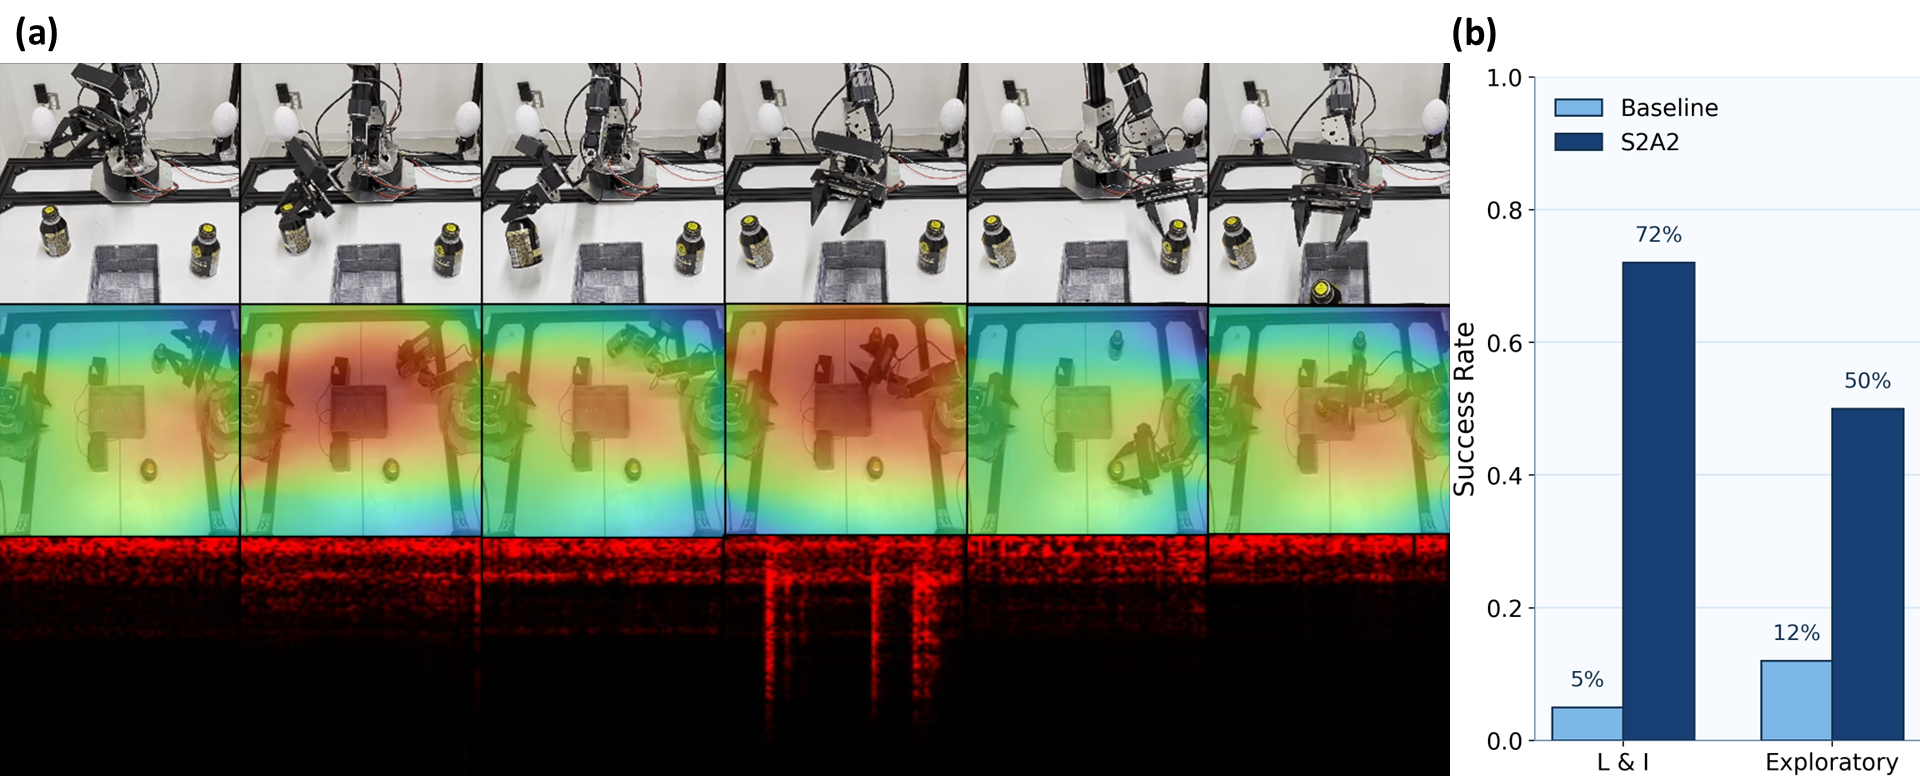
\includegraphics[keepaspectratio, width=14cm]{fig/fig5.png}
		\caption{実機実験の実行例．(a) 上段はexploratory task実行時のロボットの様子．中段はacoustic spatial mapをチャンネル方向に加算してカラーマップとして表示し，俯瞰視点のカメラ画像に重ね合わせた画像．下段はspectrogramをRGB画像のRチャンネルに入力し可視化した画像．(b) 実機実験におけるbaselineとS2A2のL\&I taskとexploratory taskの100試行におけるタスク成功率．}
		\label{fig:fig5}
	\end{figure}

\section{Conclusion}
\label{sec:conclusion}
本研究では，視覚情報のみでは操作対象や搬送先を一意に決定できない acoustic-aware manipulation tasks を導入し，音響情報を活用するマルチモーダル模倣学習フレームワーク S2A2 を提案した．

シミュレーション実験では，タスクが要求する音響的能力に応じた表現を用いることの重要性，不要な音響モダリティが性能を低下させ得ること，および音響情報の活用効率が方策アーキテクチャに依存することを示した．さらに実機実験においても，S2A2 が視覚のみのベースラインを上回る成功率を達成し，提案手法の有効性を確認した．


\section{Limitations}

本研究にはいくつかの制限がある．第一に，本研究では，音響的能力を要求する操作タスクに対して，空間的および信号的な聴覚情報を模倣学習に統合することの有効性を示すことに主眼を置いたため，実機検証は一種類のロボットおよび限定された環境で行っている点があげられる．双腕ロボットや移動ロボットを含む多様なプラットフォーム，多様な環境条件への汎用性，特に多数の異なる音源が同時に存在する環境への適用などは今後の研究である．
第二に，音響情報の活用効率は方策アーキテクチャに依存しており，特に $\pi_0$ や VQ-BeT では性能改善が限定的な条件も見られた．大規模事前学習モデルに音響情報を効果的に統合するための設計，ならびに sim-to-real 手法~\citep{multigen2025} の導入は，今後の重要な研究課題である．

\clearpage
\acknowledgments{If a paper is accepted, the final camera-ready version will (and probably should) include acknowledgments. All acknowledgments go at the end of the paper, including thanks to reviewers who gave useful comments, to colleagues who contributed to the ideas, and to funding agencies and corporate sponsors that provided financial support.}

\bibliography{main}


\end{document}